\documentclass[11pt,twocolumn,letterpaper]{article}

\usepackage{cvpr}
\usepackage{times}
\usepackage{epsfig}
\usepackage{graphicx}
\usepackage{amsmath}
\usepackage{amssymb}

% Include other packages here, before hyperref.

% If you comment hyperref and then uncomment it, you should delete
% egpaper.aux before re-running latex.  (Or just hit 'q' on the first latex
% run, let it finish, and you should be clear).
\usepackage[breaklinks=true,bookmarks=false]{hyperref}

\cvprfinalcopy % *** Uncomment this line for the final submission

\def\cvprPaperID{****} % *** Enter the CVPR Paper ID here
\def\httilde{\mbox{\tt\raisebox{-.5ex}{\symbol{126}}}}

% Pages are numbered in submission mode, and unnumbered in camera-ready
%\ifcvprfinal\pagestyle{empty}\fi
\setcounter{page}{01}
\begin{document}

%%%%%%%%% TITLE
\title{An empirical evaluation of DenseNet}

\author{Kumar Shridhar\\
Technical University Kaiserslautern\\
Kaiserslautern, Germany\\
{\tt\small k\_shridhar16.cs.uni-kl.de}
% For a paper whose authors are all at the same institution,
% omit the following lines up until the closing ``}''.
% Additional authors and addresses can be added with ``\and'',
% just like the second author.
% To save space, use either the email address or home page, not both
\and
Marcus Liwicki \\
Technical University Kaiserslautern\\
Kaiserslautern, Germany\\
{\tt\small liwicki@cs.uni-kl.de}
}

\maketitle
%\thispagestyle{empty}

%%%%%%%%% ABSTRACT
\begin{abstract}
   With the introduction of skip connections, deep neural network models can now be substantially deeper and can be trained more efficiently. This paper takes Dense Convolutional Network (DenseNet) \cite{DBLP:journals/corr/HuangLW16a}, one of the state-of-the-art architectures into account, and shows the key advantages of connecting each layer to every other layer in a feed-forward fashion. The paper also discusses all the compelling advantages of DenseNet and evaluates the performance of it's architecture on a Kaggle dataset (Dog-Breed Identification) \cite{KhoslaYaoJayadevaprakashFeiFei_FGVC2011}. Additionally, it also discusses strategies to reduce the memory consumption during training.      
\end{abstract}

%%%%%%%%% BODY TEXT
\section{Introduction}

Convolution Neural Networks (CNNs) \cite{LeCun:1989:BAH:1351079.1351090} have led to a paradigm shift in the field of Computer Vision. CNNs have recently achieved state-of-the-art results in various Image Recognition and Object Detection tasks. This has been made possible by the recent advancements in GPU hardware and availability of huge reliable datasets. Improvements in computer hardwares and network structures have enabled the training of very deep CNNs. It has also made the training process faster and more efficient. LeNet5 \cite{Lecun98gradient-basedlearning} introduced the first CNN architecture consisting of just 5 layers. Followed by which, VGGNet was introduced with 19 layers, and lately Residual Networks (ResNets) \cite{DBLP:journals/corr/HeZRS15} have surpassed the 100-layer barrier. 

\begin{figure}
	\begin{center}
		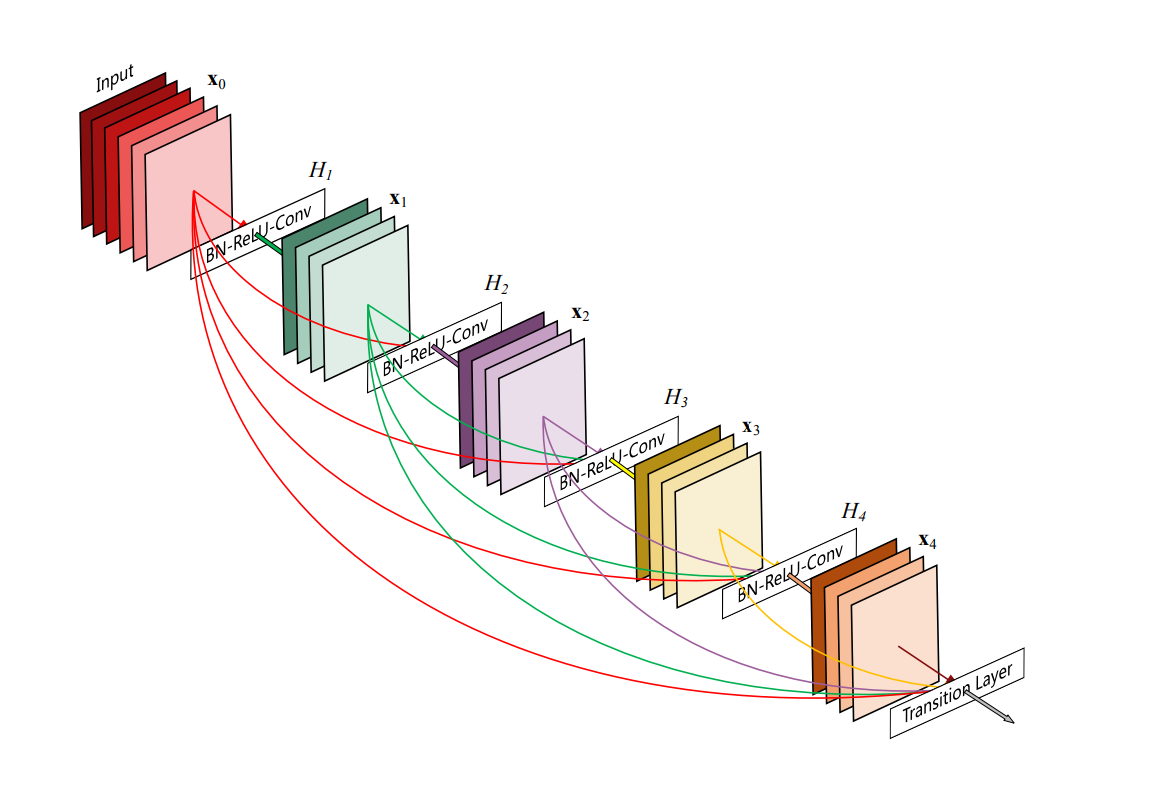
\includegraphics[width=0.8\linewidth]{image1.png}
	\end{center}
	\caption{A 5-layer dense block with a growth rate of k = 4.
		Each layer takes all preceding feature-maps as input.}
	\label{fig: image1.png}
\end{figure}

As the number of layers  in a deep neural network increases, it is accompanied by the vanishing gradient problem. ResNets \cite{DBLP:journals/corr/HeZRS15} and Highway Networks \cite{NIPS2015_5850} bypass the signal from one layer to the next via identity connections. This counters the issue of vanishing gradient. However, FractalNets (Ultra-Deep Neural Networks without Residuals) \cite{DBLP:journals/corr/LarssonMS16a}, without including any pass-through or residual connections achieve a comparable performance to deep Residual Networks. This demonstrates that residual representations may not be fundamental to the success of extremely deep convolutional neural networks.

\begin{figure*}
	\begin{center}
		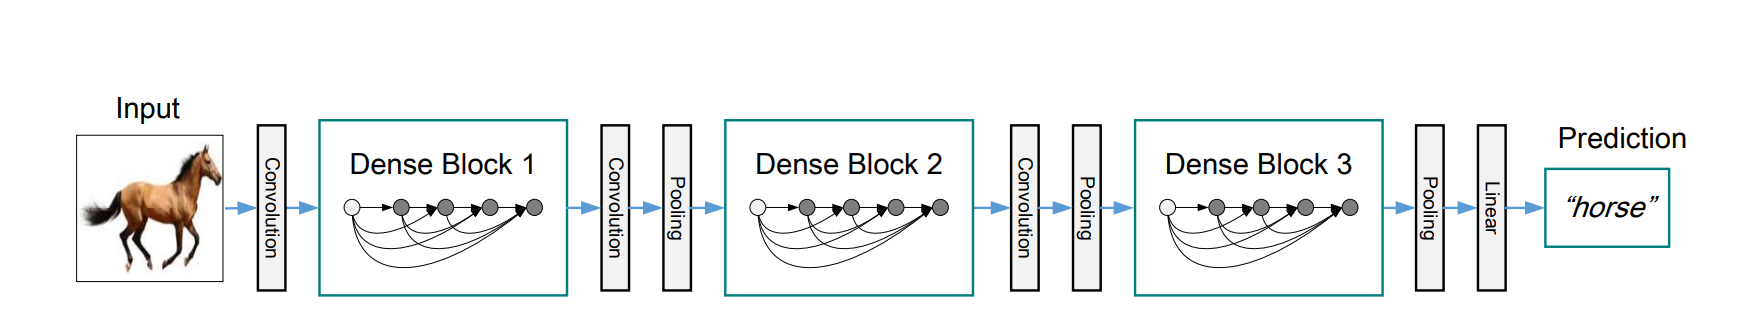
\includegraphics[width=\linewidth]{image_large.png}
	\end{center}
	\caption{A deep DenseNet with three dense blocks. The layers between two adjacent blocks are referred to as transition layers and change the feature-map sizes via convolution and pooling.}
	\label{fig: image_large.png}
\end{figure*}

Hunag \etal \cite{DBLP:journals/corr/HuangLW16a} proposed an architecture that addresses the vanishing gradient issue with a simple connectivity pattern to ensure maximum information flow between layers in the network. In this method, all layers (with matching feature-map sizes) are connected directly with each other. To preserve the feed-forward nature, each layer obtains additional inputs from all preceding layers and passes on its own feature-maps to all subsequent layers. 

Figure \ref{fig: image1.png} illustrates this layout schematically. Crucially, in contrast to ResNet, the features are never combined through summation before they are passed into a layer, instead the features are combined by concatenation. Hence, the \verb lth  layer has \verb l  inputs  consisting of the feature-maps of all preceding convolutional blocks. Its own feature-maps are passed on to all \verb L-l  subsequent layers. This introduces $L(L+1)/2$ connections in an \verb L -layer network, instead of just \verb L  connections, as in traditional architectures. Because of its dense connectivity pattern, the architecture is named as Dense Convolutional Network (DenseNet). 

%-------------------------------------------------------------------------
\section{DenseNet}
Traditional convolutional feed-forward network connects the output of one layer as the input to the next layer. ResNet \cite{DBLP:journals/corr/HeZRS15} further adds a skip connection to bypass the layers with an identity function. This helps the gradient to flow directly through the identity function. 

DenseNet on the other hand introduces direct connections from any layer to all subsequent layers. 
 Consequently, the \verb lth  layer receives the features from all preceding layers, \verb'x0, . . . , xl-1', as input:
 
 
 \begin{center}  \[x_{l} = H_{l} ([x_{0} , x_{1},  . .  .  , x_{l-1}])\] \end{center}
 
 where \verb'[x0, x1, . . . , xl-1]' refers to the concatenation of the feature-maps produced in layers \verb' 0. . . . . l-1' and \verb Hl  is any non linearity function.
 
 	 

%-------------------------------------------------------------------------


\section{Experiments}
\subsection{Performance Evaluation}


DenseNet obtains significant improvements over the state-of-the-art results on four highly competitive object recognition benchmark tasks (CIFAR-10\cite{CIFAR10}, CIFAR-100\cite{cifar100}, SVHN\cite{37648}, and ImageNet \cite{DBLP:journals/corr/RussakovskyDSKSMHKKBBF14}).
To verify that the DenseNet is as good as mentioned by the authors, it was tested on a Kaggle competition task (Dog-Breed Identification \cite{KhoslaYaoJayadevaprakashFeiFei_FGVC2011}). The results were compared with ResNet \cite{DBLP:journals/corr/HeZRS15} and InceptionNet\cite{DBLP:journals/corr/SzegedyLJSRAEVR14} that won the ImageNet \cite{DBLP:journals/corr/RussakovskyDSKSMHKKBBF14} Image Recognition Challenge in the past.

\begin{figure}
	\begin{center}
		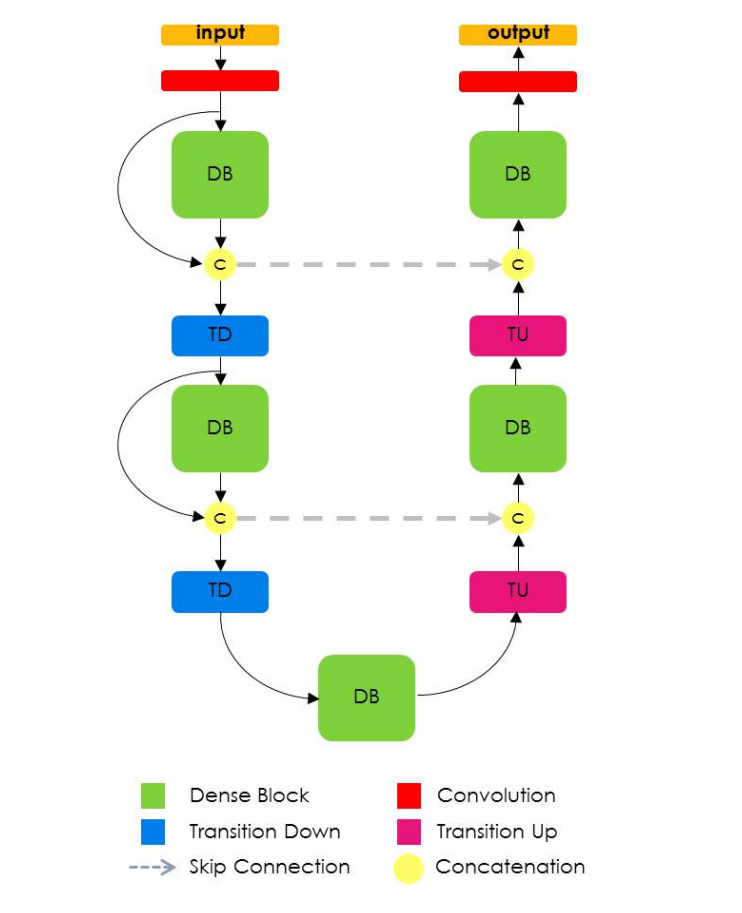
\includegraphics[width=0.8\linewidth]{image_tiramisu.png}
	\end{center}
	\caption{The architecture has 2 Transition Up (TU) blocks an 2 Transition Down (TD) blocks and gray arrows represent the skip connections from TU blocks to TD blocks.}
	\label{fig: image_tiramisu.png}
\end{figure}

As seen in Table \ref{table: table1}, DenseNet performs significantly better (89.9\% accuracy) than ResNet and InceptionNet for Dog-Breed Identification \cite{KhoslaYaoJayadevaprakashFeiFei_FGVC2011}. The performance of DenseNet was even significant than other models when no preprocessing was performed (as seen in Table \ref{table: table2}). It shows that connecting every layer's output to each subsequent layers allowed the model to learn the features more effectively. Hence, lesser data augmentation is needed for DenseNet as compared to other models for the given task. The implementation of DenseNet on Dog-Breed Identification challenge is available at: \url{https://github.com/kumar-shridhar/CNN_Architectures}.


\begin{table}
	\begin{center}
		\begin{tabular}{|l|c|}
			\hline
			Model         & Data Augmentation  \\
			\hline\hline
			ResNet50        & 88.2\% \\
			InceptionNet  & 87.4\% \\
			DenseNet      & 89.9\% \\
			\hline
		\end{tabular}
	\end{center}
	\caption{Accuracy of different model architectures on Dog-Breed Identification task.}
	\label{table: table1}
\end{table}

\begin{table}
	\begin{center}
		\begin{tabular}{|l|c|}
			\hline
			Model         & Without Data Augmentation  \\
			\hline\hline
			ResNet50      & 82.7\% \\
			InceptionNet  & 81.9\% \\
			DenseNet      & 86.4\% \\
			\hline
		\end{tabular}
	\end{center}
	\caption{Accuracy of different model architectures on Dog-Breed Identification task without data augmentation.}
	\label{table: table2}
\end{table}

Furthermore, to evaluate the performance of DenseNet, it was applied to the task of semantic segmentation. CNNs are used in the state-of-the-art methods for semantic segmentation. The architecture for most tasks perform (1) a downsampling of the image to get the features, (2) then an upsampling to get the image back, (3) and post processing like Conditional Random Field (CRF)\cite{Lafferty:2001:CRF:645530.655813} and pre processing modules like data augmentation is done to get better results. A lot of different CNN architectures were tried and DenseNet achieved the state-of-the-art results as observed by Jegou \etal \cite{DBLP:journals/corr/JegouDVRB16}. Additionally, they also achieved state of the art results on urban scene benchmark datasets, such as CamVid\cite{BrostowSFC:ECCV08} and Gatech, without any post-processing or pre-training. This shows the effectiveness of DenseNet on a task other than Image Recognition or Object Detection.

\begin{figure*}
	\begin{center}
		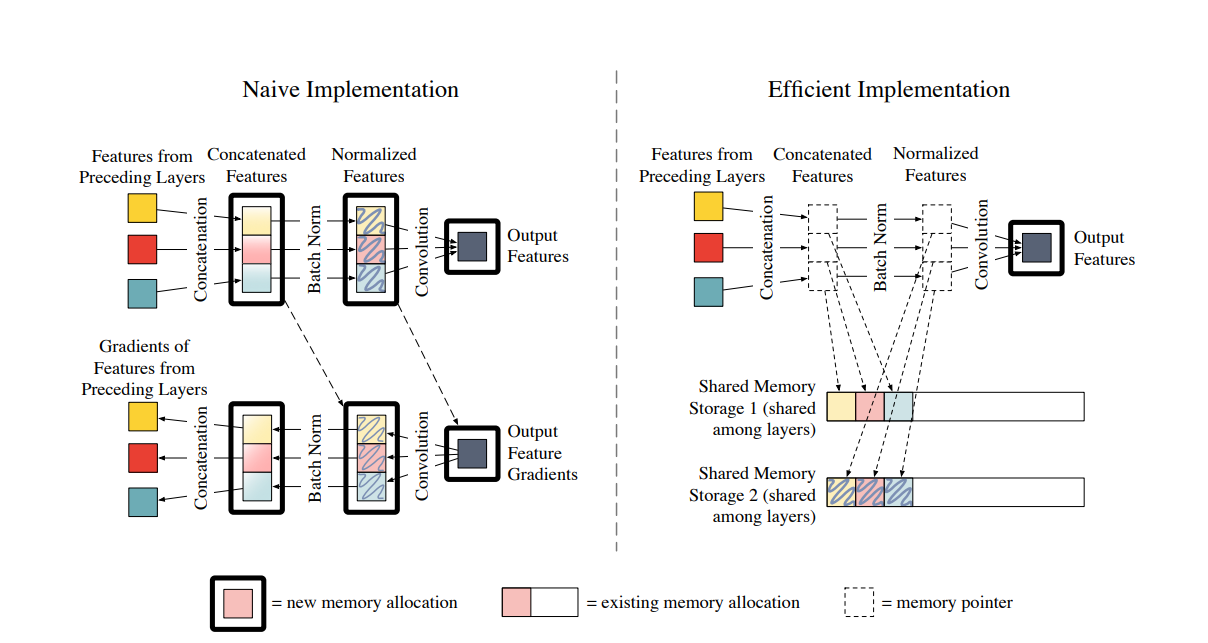
\includegraphics[width=\linewidth]{image_memory.png}
	\end{center}
	\caption{Original DenseNet implementation is on the left and its memory efficient implementation is on the right. The memory efficient implementation stores the output of the concatenation, batch normalization, and ReLU layers in temporary storage buffers, whereas the original implementation allocates new memory.}
	\label{fig: image_memory.png}
\end{figure*} 

\subsection{Memory Consumption}

DenseNet implementation in general require higher memory as seen in Figure \ref{fig: image_memory.png}. If not properly managed, pre-activation, batch normalization and contiguous convolution operations can produce feature maps that grow quadratically with the network depth. To counter these problems, the concept of Shared Memory Storage was proposed by Pleiss \etal \cite{DBLP:journals/corr/PleissCHLMW17}. During the forward pass, all intermediate outputs were assigned to shared memory blocks. During back-propagation, the concatenated and normalized features were computed dynamically.

\subsection{Training Time}

DenseNet's training time per epoch is significantly lower than ResNet and InceptionNet on the same dataset. The experiments showed a decrease of \verb 50 \% training time for DenseNet per epoch. However, to achieve the best possible results, DenseNet needs to be trained over 100 epochs as compared to 20 epochs for ResNets. This is 5 times more than the other models. So, a tradeoff exists between training time and accuracy for DenseNet. 

\section{Conclusion}

A large community of researchers believed that the approach of DenseNet was not very novel and it has been directly/indirectly applied to a lot of tasks earlier. But when observed closely, a lot of thought has been put in by the authors to  design the architecture. This has been proved by the state-of-the-art results achieved by DenseNet in a variety of Image Recognition competitions. The concept has been further tested by a series of experiments performed in this paper and by several other researchers\cite{DBLP:journals/corr/JegouDVRB16}. Overall, DenseNet is not a groundbreaking idea but the way it is implemented has achieved desired results and has proven useful for various tasks.

\section{Future Scope}

The core idea of DenseNet has opened a lot of research areas. It has already been applied in many domains (Document Analysis, Image Recognition, etc.) and it is believed it will be applied in many other areas in the near future. It would be interesting to see if an architecture similar to DenseNet can solve the need of huge amount of data for training deep learning models. The idea of DenseNet can be combined with the idea of ResNet (introduce skip connections), to avoid learning of redundant features over the layers. This is hypothesised to improve the overall training time for DenseNet and to solve problem of overfitting.

{\small
\bibliographystyle{ieee}
\bibliography{egbib}
}

\end{document}
